\documentclass[../main.tex]{subfiles}

\begin{document}

\section{Data presentation}

As a real  high-dimensional dataset, we used a genomics dataset \citep{Bessiere_Taha_Petitprez_Vandel_Marin_Brehelin_Lebre_Lecellier}.
It has a sample size of $n=19393$ and $p=531$ features.
This means that the matrix $Z$ would have $141246$ features, \ie way too many to handle directly.
The $n$ samples each represent a gene.
We chose the first response of the dataset to work, meaning one patient.
The goal of this data is to identify the active regions for the expression of different genes.
The predictive features are:
\begin{itemize}
    \item $20$ nucleotides/dinucleotides for the Core region promoter,
    \item $20$ nucleotides/dinucleotides for the DU region promoter (Distal Upstream),
    \item $20$ nucleotides/dinucleotides for the DD region promoter (Distal Downstream),
    \item $471$ motif scores computed from the Core region (JASPAR 2016 PWM scores).
\end{itemize}

\begin{definition}
The Position Weight Matrix (PWM) for nucleotide is a matrix with rows $A, T, C$ and $G$.
In each column (position) we count the number of nucleotides of each type present from our samples and
from there compute the probability distributions by dividing by the total number.
\end{definition}

The features from the three regions represent the percentages of nucleotide in the sequences divided by the length of the sequence.
The motives scores are computed as the sum over a motif $w$ of the $\log$ of:
\[\frac{\bbP(s_{i+j}\,|\, w_j)}{\bbP(s_{i+j})}\enspace,\]
where the numerator is the probability for the nucleotide at position $i+j$ of a sequence $s$ to be in position $j$ of the motif $w$.
The maximum is taken over the sequence.
This is computed from the PWM (see \Cref{sub:pwm}).

\subsection{Crash course in biology}

To understand a little more the idea of the importance of the data considered,
and why feature selection is necessary, we need to go back and understand the biological phenomenon measured.
This is in fact linked very closely to the process of going from the double helix shaped DNA gene to the protein.
This process is visualized in \Cref{fig:dna}.

\medskip

A gene is composed of nucleotide sequences.
Very simplified, it is made of a promoter region, followed by exon and introns regions.
The promoter is where the transcription is initiated, it controls how the gene is expressed.
Its Core region is known to be the one to put in place the transcription factors
while distal regions are regulatory elements mainly.
During the transcription, an helix is copied from the DNA to make the RNA from the introns and exons.
After that, the maturation of the RNA to mRNA removes the introns.
This is made in two step with the pre-mRNA to only keep the regions needed (exons) and translate some regions.
From there, we go to the cytoplasm of the cell to execute the translation.
This is where the ribosome reads the mRNA codons (groups of three nucleotides)
until reaching a "stop codon" and forms the associated amino acid chain.
The amino acid elements are linked with peptic bounds.
From there, post translational modifications are made to reach the protein,
but the polypeptic chain is the main resource for that.

\medskip
\begin{figure}[h]
    \centering
    \includegraphics[scale=.7]{transcription_dna}
    \caption{From the DNA to the protein: transcription and traduction steps. Note that in the RNA, the uracile replaces the thymine.}
    \label{fig:dna}
\end{figure}

Our response variable is the gene expression.
Quantifying it means counting the number of corresponding messenger RNA inside
the cytoplasm.
So technically it should be in $\bbN$.
However, to make it a little more Gaussian-like, a $\log$ transformation was
applied to the measurements.
Of course, since there were zeros inside the original counts,
the logarithm was not applied directly but to an $\epsilon>0$ translated quantity.
This creates a bimodal distribution (see \Cref{fig:almost_gaussian}) instead
of the unimodal Gaussian.

\begin{figure}[h]
    \centering
    \includegraphics[scale=.7]{distrib_gene_expression}
    \caption{Distribution of the gene expression for the first patient. The first peak corresponds to the shift of $\epsilon$ to avoid $-\infty$ values in the $\log$.}
    \label{fig:almost_gaussian}
\end{figure}

\subsection{Construction example for the PWM}\label{sub:pwm}
Say we have $6$ individuals with the followings nucleotide sequences:

\begin{table}[ht]
\caption{Example of imagined sequences of nucleotide available}
\centering
\begin{tabular}{|l|cccccc|}
    \hline
    sample number & 1     & 2      & 3      & 4      & 5     & 6 \\
    motif         & AATCG & ACTCC  & ATGGC  & TCGCA  & TAAGC & ATCCG\\
    \hline
\end{tabular}
\end{table}

Then the PWM is simply (with ATCG as rows from top to bottom):

\begin{align*}
    PWM &= \begin{bmatrix}
        \frac{\sharp \{A\text{ in first place}\}}{6} & \frac{\sharp \{A\text{ in second place}\}}{6} & \frac{\sharp \{A\text{ in third place}\}}{6} & \frac{\sharp \{A\text{ in fourth place}\}}{6} & \frac{\sharp \{A\text{ in fifth place}\}}{6} \\
        \frac{\sharp \{T\text{ in first place}\}}{6} & \frac{\sharp \{T\text{ in second place}\}}{6} & \frac{\sharp \{T\text{ in third place}\}}{6} & \frac{\sharp \{T\text{ in fourth place}\}}{6} & \frac{\sharp \{T\text{ in fifth place}\}}{6} \\
        \frac{\sharp \{C\text{ in first place}\}}{6} & \frac{\sharp \{C\text{ in second place}\}}{6} & \frac{\sharp \{C\text{ in third place}\}}{6} & \frac{\sharp \{C\text{ in fourth place}\}}{6} & \frac{\sharp \{C\text{ in fifth place}\}}{6} \\
        \frac{\sharp \{G\text{ in first place}\}}{6} & \frac{\sharp \{G\text{ in second place}\}}{6} & \frac{\sharp \{G\text{ in third place}\}}{6} & \frac{\sharp \{G\text{ in fourth place}\}}{6} & \frac{\sharp \{G\text{ in fifth place}\}}{6}
    \end{bmatrix} \\
  & \simeq \begin{bmatrix}
    4/6\simeq 0.67 & 2/6\simeq 0.33 & 1/6\simeq 0.17 & 0 & 1/6\simeq 0.17\\
    0.33 & 0.33 & 0.33 & 0 & 0 \\
    0 & 0.33 & 0.17 & 0.67 & 0.5 \\
    0 & 0 & 0.33 & 0.33 & 0.33
\end{bmatrix}\enspace.
\end{align*}

From there, then a posteriori,
\begin{align*}
\bbP(ACCGA\,|\, w)
&= \bbP(\{A\text{ in first place}\}\,|\, PWM)\times \bbP(\{C\text{ in second place}\}\,|\, PWM)\dots \bbP(\{A\text{ in fifth place}\}\,|\, PWM) \\
&\simeq 0.67\times 0.33\times 0.17\times 0.33\times 0.17\enspace.
\end{align*}

\subsection{Numerical stability}\label{sub:num_stability}

With small visualizations, we can already foresee the issues we will face and discuss more in \Cref{sub:num_stability}.
For example, we can look at a kernel density estimation of the distribution of
the first five features of our data and their joined distribution.
\begin{figure}[ht]
    \centering
    \includegraphics[scale=.5]{5_features_pairgrid}
    \caption{Estimated densities and joined densities of the first five features
    in Core region.}
    \label{5coreplots}
\end{figure}

\Cref{5coreplots} already shows us highly correlated features.
However, we also notice that the features are unimodal, bell-shaped distributed.
With \Cref{fig:gram_genom} we will see that it is not only a phenomenon on the
first features but on the all first $60$ features (the three regions).
For the PMW scores, with \Cref{fig:pmw} we see that they are mainly close to one,
mostly because what is used is the $\max$ of the sum of logs.
This property is verified along all the $471$ features.

\begin{figure}[ht]
    \centering
    \includegraphics[scale=.8]{boxenplot_genom.pdf}
    \caption{Boxplot with the $10$ quantiles of the features $80$ to $90$
    (motif scores).}
    \label{fig:pmw}
\end{figure}

We apply the usual way to preprocess the data $X \in \bbR^{n\times p}$ for a dataset:
the standardization from \Cref{eq:standard}:
\begin{align} \label{eq:standard}
    \frac{X - \mu}{\sigma}\enspace,
\end{align}
with $\mu$ and $\sigma$ the mean and standard-deviation of $X$.
We can look at the numerical stability of our data after standardization.
One way to measure this is to consider the condition number of the data.
\begin{definition}
The condition number of a rectangular matrix $A$ denoted $\kappa(A)$ is:
\[\kappa(A) = \bnorm{A}\bnorm{A^+}\enspace,\]
where $A^+$ is the pseudo-inverse of $A$. Using the $2-$norm,
\[\kappa(A) = \frac{\sigma_{\max}}{\sigma_{\min}}\enspace,\]
the ratio of the largest and smallest singular values.
\end{definition}

With simulated aforementioned data from Gaussian distributions, $\kappa(X)\simeq 1.7$ which is
a very good condition number as the best possible is $\kappa(\Id)=1$.
And all the condition numbers of the blocks of the associated matrix were below $2$.
With \Cref{fig:cond_genom} we can look at the condition number of each block of
the matrix $Z$ for the genomics dataset. And for the first $60$ blocks it is way too big.
\begin{figure}[ht]
    \centering
    \includegraphics[scale=.5]{condition_number_genom}
    \caption{Condition number of the blocks of the interaction matrix with genomics data.}
    \label{fig:cond_genom}
\end{figure}

\medskip

In fact, it is not even precise to talk about $10^{15}$ as a condition number
for $Z_{\branch{q}{1}}$ as $\sigma_{\min} < 10^{-20}$ so we have already reached
(by far) the zero-machine precision.
If the smallest singular value is so close to zero, then the columns are almost
linearly dependant.
 \Cref{fig:gram_genom} represents the Gram matrix of the genomics dataset,
 $\Sigma=\nicefrac{X^\top X}{n}$.
As we can see, the first $60$ features have indeed a different behaviour and
there are some very highly correlated features (in absolute value).
This alone justifies the use of the Elastic-Net, the $\ell_2$ norm being
used as a regulator.
\begin{figure}[ht]
    \centering
	\begin{subfigure}{.45\textwidth}
		\centering
		\includegraphics[width=.8\textwidth, clip, trim={1.2cm 0 1cm 0}]{Gram_matrix_genom}
		\subcaption{All features}
	\end{subfigure} \hspace{.1cm}
	\begin{subfigure}{.45\textwidth}
		\centering
		\includegraphics[width=.8\textwidth, clip, trim={1.2cm 0 1cm 0}]{Gram_matrix_genom_60}
		\subcaption{First $60$ features of the genomics dataset}
	\end{subfigure}
	\caption{Gram matrices of the genomics dataset.}
    \label{fig:gram_genom}
\end{figure}

\section{Running solvers on the genomics dataset} \label{sec:solv_genom}

When working with such data, it is not possible to consider one set of penalties
directly.
So what we need to look at is the time taken to complete a whole path.
And it is interesting to consider different values of $\epsilon>0$ as stopping
values for \Cref{eq:eps_kkt}, the KKT criterion.
There are also two new elements to consider:
\begin{itemize}
    \item because we are working with a path, we can consider to use warm starts.
    Meaning that the path is computed from the largest $\ell_1$ penalty to the smallest.
    And when starting to solve the problem with the next penalty, instead of starting
    from the zero-solution, we can use the solution we previously ended up with.
    \item to help with numerical stability on the GPU methods, we recompute every $100$ epochs the residuals $r=X\beta + Z\Theta - y$.
    This is done for the first penalty only (to have a solver that converged when
    the warm start is tried in the accelerated version) or for all the penalties \ow.
\end{itemize}
\begin{figure}[ht]
    \centering
    \includegraphics[scale=.45]{barplot_genom_factor20}
    \caption{Barplot of the ratio of time taken to compute a full path \wrt
    vanilla CD method for different precision.
    We use the KKT criterion on the genomics dataset.
    As $\ell_1$ penalty, $10$ $\log$-spaced values on a grid
     from $\lambda_{\max}$ to $\lambda_{\max}/100$ are used.
     The $\ell_2$ penalty is set to $20\lambda_{\ell_1, \max}$.
     All solvers reached convergence criterion.}
    \label{fig:barplots_genom}
\end{figure}

\Cref{fig:barplots_genom} shows that CD methods are quick to find where to go
to reach the $10^{-2}$ precision.
However as the $\epsilon$ becomes smaller, CBPG based methods perform better.
It is worth noticing that using a warm start and recompute residuals for all
penalties lead to the same performance results.
So the proximal gradient descent based algorithms with GPU can indeed become
competitive against Coordinate Descent.

\end{document}
